\documentclass[12pt,a4paper]{report}
\usepackage[T2A]{fontenc}
\usepackage[utf8]{inputenc}
\usepackage[russian]{babel}
\usepackage[LGRgreek]{mathastext}
\usepackage{graphicx, setspace, multirow, amsmath}
\usepackage[table,xcdraw]{xcolor}
\usepackage{slashbox}

\usepackage[
top = 1.25cm,
bottom = 2.0cm]{geometry}

\makeatletter
\newcommand{\mathleft}{\@fleqntrue\@mathmargin0pt}
\newcommand{\mathcenter}{\@fleqnfalse}
\makeatother

\begin{document}
\begin{titlepage}
	\centering
    % HEADER
	{
        \scshape
        Федеральное государственное автономное образовательное учреждение высшего образования
        \par
        \textbf{«Научно-образовательная корпорация ИТМО»}
        \par
        \vspace*{1cm}
        Факультет Программной Инженерии и Компьютерной Техники
        \par
    }
    % LOGO
    \vspace*{0.6cm}
    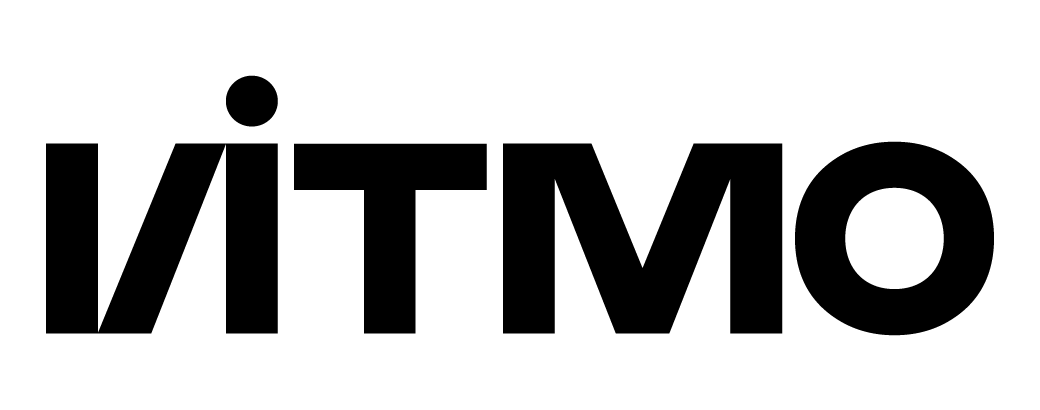
\includegraphics[width=\textwidth]{logo.png}
    % LAB INFO
    {
        \Large
        \textbf{Курсовая работа\\ <<Синтез комбинаторных схем>>\\ Часть №2}
        \par 
        \normalsize
        \vspace*{0.75cm}
        \textbf{Вариант 78}
        \par
    }
    \vfill
    % СREDITS
    \hfill\begin{minipage}{\dimexpr\textwidth-7.8cm}
        \textbf{Выполнил:}\par
        Степанов Арсений Алексеевич\par
        \vspace*{0.15cm}
        \textbf{Группа:}\par
        P3109\par
        \vspace*{0.15cm}
        \textbf{Преподаватель:}\par
        Поляков Владимир Иванович\par
    \end{minipage}
    \vfill
    Санкт-Петербург, \the\year{}г. 
\end{titlepage}
\onehalfspacing
\mathleft
\section*{Определение функции}
$C=A+2(-B)$\\
Разрядность операндов: A -- 4(2) бита, B -- 0(2) битов, C -- 4 бита\\
На вход передаётся специальный бит $y$, который переключает режим работы схемы, таким образом:
\begin{equation*}
    \begin{cases}
        y=0,\;C=A+2\\
        y=1,\;C=A-B\\
    \end{cases}
\end{equation*}
Флаг переноса выставляется в специально отведённый бит $p$\\
5 бит на вход (1 сигнальный и 4 знаковых бита) и 5 бит на выход (1 бит для флага переноса и 4 знаковых бита) схемы
\section*{Таблица истинности}
\begin{tabular}{|c|cc|cc||c|cccc|}
    \hline
    \multicolumn{5}{|c||}{Входные сигналы} & \multicolumn{5}{c|}{Выходные сигналы}\\
    \hline
    $y$ & $a_1$ & $a_2$ & $b_1$ & $b_2$ & $p$ & $c_1$ & $c_2$ & $c_3$ & $c_4$\\
    \hline
    $0$ & $0$ & $0$ & $0$ & $0$ & $0$ & $0$ & $0$ & $1$ & $0$\\
    \hline
    $0$ & $0$ & $0$ & $0$ & $1$ & $0$ & $0$ & $0$ & $1$ & $1$\\
    \hline
    $0$ & $0$ & $0$ & $1$ & $0$ & $0$ & $0$ & $1$ & $0$ & $0$\\
    \hline
    $0$ & $0$ & $0$ & $1$ & $1$ & $0$ & $0$ & $1$ & $0$ & $1$\\
    \hline
    $0$ & $0$ & $1$ & $0$ & $0$ & $0$ & $0$ & $1$ & $1$ & $0$\\
    \hline
    $0$ & $0$ & $1$ & $0$ & $1$ & $0$ & $0$ & $1$ & $1$ & $1$\\
    \hline
    $0$ & $0$ & $1$ & $1$ & $0$ & $0$ & $1$ & $0$ & $0$ & $0$\\
    \hline
    $0$ & $0$ & $1$ & $1$ & $1$ & $0$ & $1$ & $0$ & $0$ & $1$\\
    \hline
    $0$ & $1$ & $0$ & $0$ & $0$ & $0$ & $1$ & $0$ & $1$ & $0$\\
    \hline
    $0$ & $1$ & $0$ & $0$ & $1$ & $0$ & $1$ & $0$ & $1$ & $1$\\
    \hline
    $0$ & $1$ & $0$ & $1$ & $0$ & $0$ & $1$ & $1$ & $0$ & $0$\\
    \hline
    $0$ & $1$ & $0$ & $1$ & $1$ & $0$ & $1$ & $1$ & $0$ & $1$\\
    \hline
    $0$ & $1$ & $1$ & $0$ & $0$ & $0$ & $1$ & $1$ & $1$ & $0$\\
    \hline
    $0$ & $1$ & $1$ & $0$ & $1$ & $0$ & $1$ & $1$ & $1$ & $1$\\
    \hline
    $0$ & $1$ & $1$ & $1$ & $0$ & $1$ & $0$ & $0$ & $0$ & $0$\\
    \hline
    $0$ & $1$ & $1$ & $1$ & $1$ & $1$ & $0$ & $0$ & $0$ & $1$\\
    \hline
    $1$ & $0$ & $0$ & $0$ & $0$ & $0$ & $0$ & $0$ & $0$ & $0$\\
    \hline
    $1$ & $0$ & $0$ & $0$ & $1$ & $1$ & $1$ & $1$ & $1$ & $1$\\
    \hline
    $1$ & $0$ & $0$ & $1$ & $0$ & $1$ & $1$ & $1$ & $1$ & $0$\\
    \hline
    $1$ & $0$ & $0$ & $1$ & $1$ & $1$ & $1$ & $1$ & $0$ & $1$\\
    \hline
    $1$ & $0$ & $1$ & $0$ & $0$ & $0$ & $0$ & $0$ & $0$ & $1$\\
    \hline
    $1$ & $0$ & $1$ & $0$ & $1$ & $0$ & $0$ & $0$ & $0$ & $0$\\
    \hline
    $1$ & $0$ & $1$ & $1$ & $0$ & $1$ & $1$ & $1$ & $1$ & $1$\\
    \hline
    $1$ & $0$ & $1$ & $1$ & $1$ & $1$ & $1$ & $1$ & $1$ & $0$\\
    \hline
    $1$ & $1$ & $0$ & $0$ & $0$ & $0$ & $0$ & $0$ & $1$ & $0$\\
    \hline
    $1$ & $1$ & $0$ & $0$ & $1$ & $0$ & $0$ & $0$ & $0$ & $1$\\
    \hline
    $1$ & $1$ & $0$ & $1$ & $0$ & $0$ & $0$ & $0$ & $0$ & $0$\\
    \hline
    $1$ & $1$ & $0$ & $1$ & $1$ & $1$ & $1$ & $1$ & $1$ & $1$\\
    \hline
    $1$ & $1$ & $1$ & $0$ & $0$ & $0$ & $0$ & $0$ & $1$ & $1$\\
    \hline
    $1$ & $1$ & $1$ & $0$ & $1$ & $0$ & $0$ & $0$ & $1$ & $0$\\
    \hline
    $1$ & $1$ & $1$ & $1$ & $0$ & $0$ & $0$ & $0$ & $0$ & $1$\\
    \hline
    $1$ & $1$ & $1$ & $1$ & $1$ & $0$ & $0$ & $0$ & $0$ & $0$\\
    \hline
\end{tabular}
\newpage
\section*{Минимизация на картах Карно}
\includegraphics[width=12cm]{karno_p.png}\\
$p=\overline{y}\,a_1\,a_2\,b_1 \lor y\,\overline{a_1}\,\overline{a_2}\,b_2 \lor y\,\overline{a_2}\,b_1\,b_2 \lor y\,\overline{a_1}\,b_1$\\
$S_Q=19$\\
\hfill\break
\includegraphics[width=12cm]{karno_c1.png}\\
$c_1=y\,\overline{a_2}\,b_1\,b_2 \lor y\,\overline{a_1}\,\overline{a_2}\,b_2 \lor \overline{y}\,a_1\,\overline{a_2} \lor \overline{y}\,a_1\,\overline{b_1} \lor \overline{a_1}\,a_2\,b_1 \lor y\,\overline{a_1}\,b_1$\\
$S_Q=26$\\
\hfill\break
\includegraphics[width=12cm]{karno_c2.png}\\
$c_2=y\,\overline{a_2}\,b_1\,b_2 \lor y\,\overline{a_1}\,\overline{a_2}\,b_2 \lor  \overline{y}\,a_2\,\overline{b_1} \lor \overline{y}\,\overline{a_2}\,b_1 \lor y\,\overline{a_1}\,b_1$\\
$S_Q=22$\\
\hfill\break
\includegraphics[width=12cm]{karno_c3.png}\\
$c_3=y\,a_1\,\overline{a_2}\,b_1\,b_2 \lor \overline{a_1}\,\overline{a_2}\,\overline{b_1}\,b_2 \lor y\,\overline{a_1}\,b_1\,\overline{b_2} \lor y\,\overline{a_1}\,a_2\,b_1 \lor a_1\,a_2\,\overline{b_1} \lor a_1\,\overline{b_1}\,\overline{b_2} \lor \overline{y}\,\overline{b_1}$\\
$S_Q=32$\\
\hfill\break
\includegraphics[width=12cm]{karno_c4.png}\\
$c_4=y\,a_2\,\overline{b_2} \lor \overline{a_2}\,b_2 \lor \overline{y}\,b_2$\\
$S_Q=10$\\
\newpage
\section*{Преобразование системы полученных функций}
\subsubsection*{Исходная система}
\begin{equation*}
    \begin{cases}
        p=\overline{y}\,a_1\,a_2\,b_1 \lor y\,\overline{a_1}\,\overline{a_2}\,b_2 \lor y\,\overline{a_2}\,b_1\,b_2 \lor y\,\overline{a_1}\,b_1\\
        c_1=y\,\overline{a_2}\,b_1\,b_2 \lor y\,\overline{a_1}\,\overline{a_2}\,b_2 \lor \overline{y}\,a_1\,\overline{a_2} \lor \overline{y}\,a_1\,\overline{b_1} \lor \overline{a_1}\,a_2\,b_1 \lor y\,\overline{a_1}\,b_1\\
        c_2=y\,\overline{a_2}\,b_1\,b_2 \lor y\,\overline{a_1}\,\overline{a_2}\,b_2 \lor  \overline{y}\,a_2\,\overline{b_1} \lor \overline{y}\,\overline{a_2}\,b_1 \lor y\,\overline{a_1}\,b_1\\
        c_3=y\,a_1\,\overline{a_2}\,b_1\,b_2 \lor \overline{a_1}\,\overline{a_2}\,\overline{b_1}\,b_2 \lor y\,\overline{a_1}\,b_1\,\overline{b_2} \lor y\,\overline{a_1}\,a_2\,b_1 \lor a_1\,a_2\,\overline{b_1} \lor a_1\,\overline{b_1}\,\overline{b_2} \lor \overline{y}\,\overline{b_1}\\
        c_4=y\,a_2\,\overline{b_2} \lor \overline{a_2}\,b_2 \lor \overline{y}\,b_2\\
    \end{cases}
\end{equation*}
$S_Q=S_Q^p+S_Q^{c_1}+S_Q^{c_2}+S_Q^{c_3}+S_Q^{c_4}=19+26+22+32+10=109$
\subsubsection*{Факторизация}
\begin{equation*}
    \begin{cases}
        p=\overline{y}\,a_1\,a_2\,b_1 \lor y\,(\overline{a_2}\,b_2\,(\overline{a_1} \lor b_1) \lor \overline{a_1}\,b_1)\\
        c_1=y\,(\overline{a_2}\,b_2\,(\overline{a_1} \lor b_1) \lor \overline{a_1}\,b_1) \lor \overline{y}\,a_1\,(\overline{a_2}\lor\overline{b_1})\lor \overline{a_1}\,a_2\,b_1\\
        c_2=y\,(\overline{a_2}\,b_2\,(\overline{a_1} \lor b_1) \lor \overline{a_1}\,b_1) \lor \overline{y}\,(\overline{a_2}\,b_1 \lor a_2\,\overline{b_1})\\
        c_3=\overline{b_1}\,(\overline{a_1}\,\overline{a_2}\,b_2 \lor a_1\,a_2 \lor a_1\,\overline{b_2} \lor \overline{y}) \lor y\,b_1\,(a_1\,\overline{a_2}\,b_2\lor\overline{a_1}\,\overline{b_2}\lor\overline{a_1}\,a_2)\\
        c_4=y\,a_2\,\overline{b_2} \lor \overline{a_2}\,b_2 \lor \overline{y}\,b_2\\
    \end{cases}
\end{equation*}
$S_Q=S_Q^p+S_Q^{c_1}+S_Q^{c_2}+S_Q^{c_3}+S_Q^{c_4}=17+22+21+28+10=98$
\subsubsection*{Декомпозиция}
\begin{tabular}{ll}
    $\varphi_1=y\,(\overline{a_2}\,b_2\,(\overline{a_1} \lor b_1) \lor \overline{a_1}\,b_1)$ & $\overline{\varphi_1}=\overline{y} \lor ((a_2 \lor \overline{b_2} \lor \overline{a_1}\,\overline{b_2})\land (\overline{a_1} \lor \overline{b_1}))$\\
    $\varphi_2=a_2\,b_1$ & $\overline{\varphi_2}=\overline{a_2}\lor\overline{b_1}$\\
    $\varphi_3=\overline{a_2}\,b_2$ & $\overline{\varphi_3}=a_2\lor\overline{b_2}$
\end{tabular}

\begin{equation*}
    \begin{cases}
        \varphi_1=y\,(\varphi_3\,(\overline{a_1} \lor b_1) \lor \overline{a_1}\,b_1)\\
        \varphi_2=a_2\,b_1\\
        \varphi_3=\overline{a_2}\,b_2\\
        p=\overline{y}\,a_1\,\varphi_2 \lor \varphi_1\\
        c_1=\varphi_1 \lor \overline{y}\,a_1\,\overline{\varphi_2}\lor \overline{a_1}\,\varphi_2\\
        c_2=\varphi_1 \lor \overline{y}\,(\overline{a_2}\,b_1 \lor a_2\,\overline{b_1})\\
        c_3=\overline{b_1}\,(\overline{a_1}\,\varphi_3 \lor a_1\,\overline{\varphi_3} \lor \overline{y}) \lor y\,b_1\,(a_1\,\varphi_3\lor\overline{a_1}\,\overline{b_2}\lor\overline{a_1}\,a_2)\\
        c_4=y\,a_2\,\overline{b_2} \lor \varphi_3 \lor \overline{y}\,b_2\\
    \end{cases}
\end{equation*}
$S_Q=S_Q^{\varphi_1}+S_Q^{\varphi_2}+S_Q^{\varphi_3}+S_Q^p+S_Q^{c_1}+S_Q^{c_2}+S_Q^{c_3}+S_Q^{c_4}=8+2+2+5+8+10+20+8+3=66$
\newpage
\section*{Синтез комбинационной схемы в булевом базисе}
Анализировать схему будем на наборе аргументов $f(0, 1, 0, 1, 0) = (0, 1, 1, 0, 0)$\\
\hfill\break
\includegraphics[width=14cm]{schema.png}\\
\hfill\break
$S_q=66$, $T=6\tau$
\end{document}

